% Training Curves for 3D-GCN
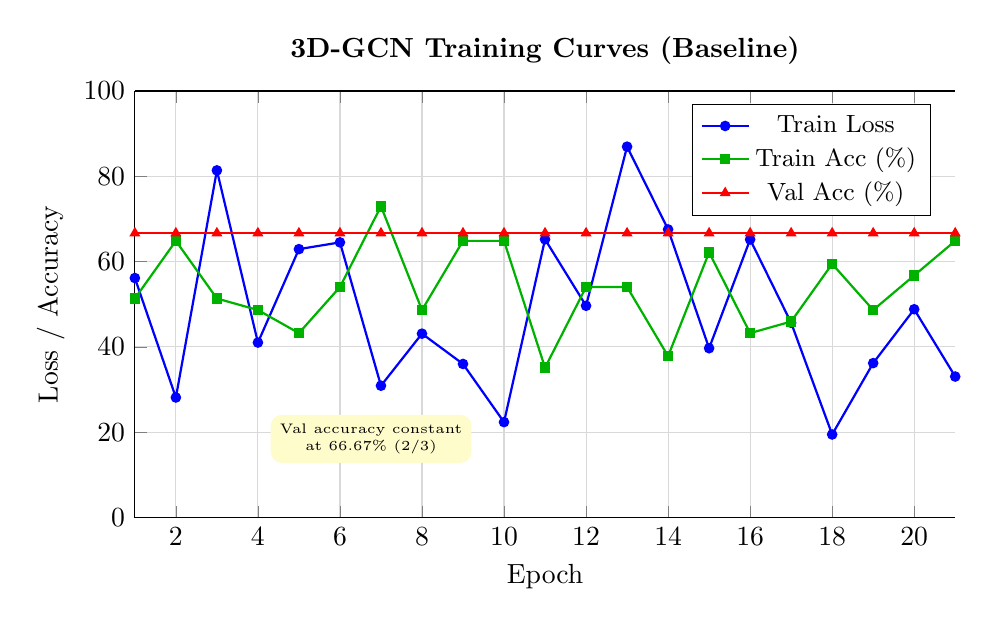
\begin{tikzpicture}
\begin{axis}[
    width=12cm,
    height=7cm,
    xlabel={Epoch},
    ylabel={Loss / Accuracy},
    xmin=1, xmax=21,
    ymin=0, ymax=100,
    legend pos=north east,
    legend style={font=\small},
    grid=major,
    grid style={gray!30},
    title={\textbf{3D-GCN Training Curves (Baseline)}},
    title style={font=\bfseries},
    axis y line*=left,
]

% Training Loss (scaled for visibility)
\addplot[
    thick,
    blue,
    mark=*,
    mark size=1.5pt
] coordinates {
    (1, 56.15) (2, 28.15) (3, 81.38) (4, 41.02) (5, 62.92)
    (6, 64.51) (7, 30.91) (8, 43.11) (9, 36.01) (10, 22.38)
    (11, 65.22) (12, 49.65) (13, 86.94) (14, 67.54) (15, 39.70)
    (16, 65.19) (17, 45.66) (18, 19.48) (19, 36.21) (20, 48.83)
    (21, 33.06)
};
\addlegendentry{Train Loss}

% Training Accuracy (scaled to 0-100)
\addplot[
    thick,
    green!70!black,
    mark=square*,
    mark size=1.5pt
] coordinates {
    (1, 51.35) (2, 64.86) (3, 51.35) (4, 48.65) (5, 43.24)
    (6, 54.05) (7, 72.97) (8, 48.65) (9, 64.86) (10, 64.86)
    (11, 35.14) (12, 54.05) (13, 54.05) (14, 37.84) (15, 62.16)
    (16, 43.24) (17, 45.95) (18, 59.46) (19, 48.65) (20, 56.76)
    (21, 64.86)
};
\addlegendentry{Train Acc (\%)}

% Validation Accuracy (constant)
\addplot[
    thick,
    red,
    mark=triangle*,
    mark size=1.5pt
] coordinates {
    (1, 66.67) (2, 66.67) (3, 66.67) (4, 66.67) (5, 66.67)
    (6, 66.67) (7, 66.67) (8, 66.67) (9, 66.67) (10, 66.67)
    (11, 66.67) (12, 66.67) (13, 66.67) (14, 66.67) (15, 66.67)
    (16, 66.67) (17, 66.67) (18, 66.67) (19, 66.67) (20, 66.67)
    (21, 66.67)
};
\addlegendentry{Val Acc (\%)}

\end{axis}

% Annotation
\node[font=\tiny, fill=yellow!20, rounded corners, align=center] at (3, 1) {
    Val accuracy constant\\
    at 66.67\% (2/3)
};

\end{tikzpicture}




